% Compile with XeLaTeX or LuaLaTeX
\documentclass[10pt,a4paper]{article}
\usepackage{xcolor}
\usepackage{titlesec}
\usepackage{fontspec}
\defaultfontfeatures{Mapping=tex-text}
\usepackage{xunicode}
\usepackage{xltxtra}
\usepackage{polyglossia}
\usepackage{indentfirst}             % 段首缩进

\setdefaultlanguage{english}
% 设置字体
\setsansfont{Calibri}
\setmainfont[BoldFont=SimHei]{STKaiti}
\usepackage{amsmath}
\usepackage{amsfonts}
\usepackage{amssymb}
\usepackage{graphicx}
% 设置页边距
%\usepackage[left=2cm,right=2cm,top=2cm,bottom=2cm]{geometry}
% MATLAB代码插入包
\usepackage{listings}
\usepackage[framed,numbered,autolinebreaks,useliterate]{mcode}
% 新定义字体
\newfontfamily\song{SimSun}          % 宋体
\newfontfamily\hei{SimHei}           % 黑体
\XeTeXlinebreaklocale "zh"           % 中文断行

% Define light and dark Microsoft blue colours
\definecolor{MSBlue}{rgb}{.204,.353,.541}
\definecolor{MSLightBlue}{rgb}{.31,.506,.741}
% Define a new fontfamily for the subsubsection font
% Don't use \fontspec directly to change the font
\newfontfamily\subsubsectionfont[Color=MSLightBlue]{Times New Roman}
% Set formats for each heading level
\titleformat*{\section}{\Large\bfseries\sffamily\color{MSBlue}}
\titleformat*{\subsection}{\large\bfseries\sffamily\color{MSLightBlue}\song}
\titleformat*{\subsubsection}{\itshape\subsubsectionfont}

\author{邸明轩\footnote{email: mingxuandi@163.com}\\[2ex]
	\\[2ex]}
\title{牛熊市试验报告 \uppercase\expandafter{\romannumeral3}:特征工程}
\date{08, 16, 2016}
\begin{document}
	
	%%%% 段落首行缩进两个字 %%%%
	\makeatletter
	\let\@afterindentfalse\@afterindenttrue
	\@afterindenttrue
	\makeatother
	\setlength{\parindent}{2em}  %中文缩进两个汉字位
	
	\maketitle
	
	\section{Explain }
	数据和特征决定了机器学习的上限,而统计学习等机器学习模型和算法只是逼近这个上限而已。那特征工程到底是什么呢?顾名思义,其本质是一项工程活动,目的是最大限度地从原始数据中提取特征以供算法和模型使用。
	\begin{figure}[t]
		\centering
		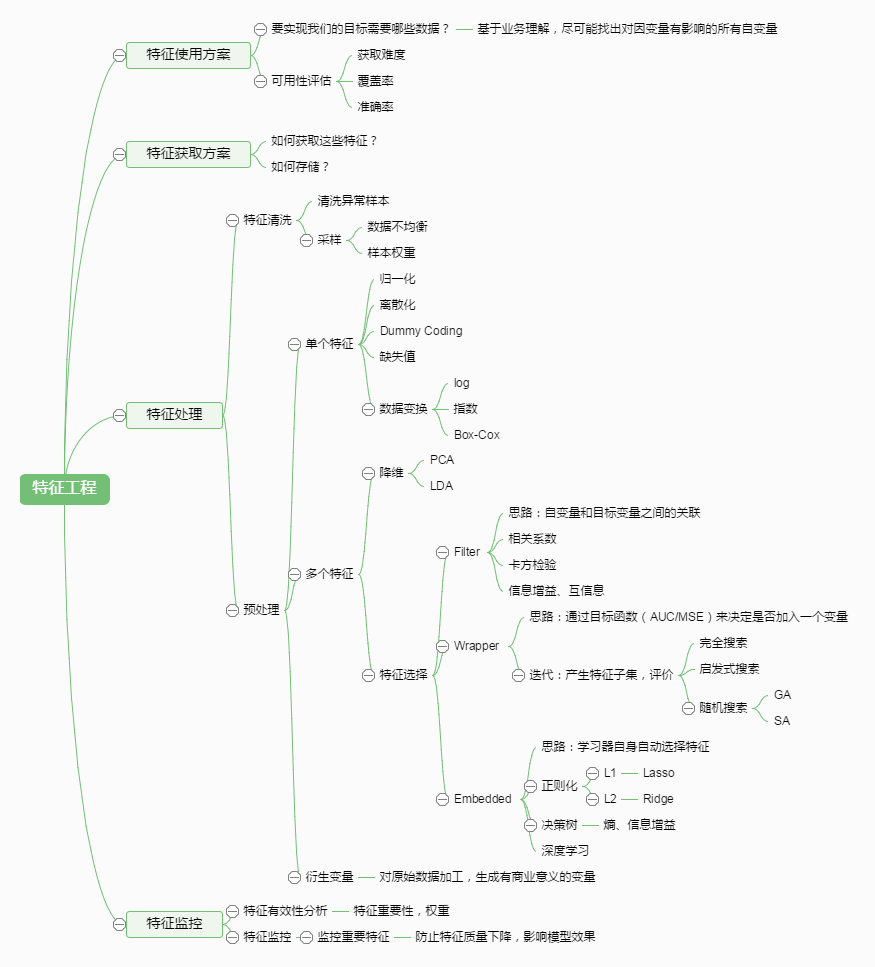
\includegraphics[width=0.9\linewidth]{特征工程说明.jpg}
		\caption{特征工程的流程图,不感兴趣可以略过}
		\label{fig1}
	\end{figure}
	\section{Result }
\noindent 模型:Logistic Regression分类器 + L1范数 + L2范数\\
目前使用了月度的指标,可以理解为每月最后一个交易日的指标,所以也是稀疏的(每月一次)的日指标。\\

\noindent 实验一:标准化\\
标准化需要计算特征的均值和标准差,公式表达为:
\begin{equation}
\label{eq:u0}
\begin{aligned}
{x}'= \frac{x-Min}{Max-Min}
\end{aligned}
\end{equation}\\
F1准确率: 0.0.6278 \\

\noindent 实验二:归一化\\
对特征做归一化处理,利用两个最值进行缩放,公式表达为:
\begin{equation}
\label{eq:u0}
\begin{aligned}
{x}'= \frac{x-\bar{X}}{S}\\
\end{aligned}
\end{equation}\\
F1准确率: 0.6371\\
		
		
\noindent  实验n:数据变换\\

常见的数据变换有基于多项式的、基于指数函数的、基于对数函数的. 2维特征的2阶多项式特征如下:$[1, a, b, a^2, ab, b^2].$
		
\noindent  实验四:\\
特征:实验二特征 + 前一季度归母净利 + 前一季度归母权益 + 前一季度ROE,共九个特征。(当季无法获取当季$roe$等指标,所以使用了前一季度指标)\\
F1准确率: 0.6312 (0.1164)\\

\noindent  实验五:\\
特征:实验四特征 + 票据转贴利率 + 人民币名义有效汇率\\
F1准确率: 0.6366 (0.1073)\\

%	\section{Criterion }
%	
%		\begin{equation}
%			\label{eq:u0}
%			\begin{aligned}
%				Score=E+ \alpha  \sum_{i=0}^{2}k_{i}p_{i}(x)logk_{i}p_{i}(x)
%			\end{aligned}
%		\end{equation}
	
\end{document}